
%% bare_conf.tex
%% V1.4b
%% 2015/08/26
%% by Michael Shell
%% See:
%% http://www.michaelshell.org/
%% for current contact information.
%%
%% This is a skeleton file demonstrating the use of IEEEtran.cls
%% (requires IEEEtran.cls version 1.8b or later) with an IEEE
%% conference paper.
%%
%% Support sites:
%% http://www.michaelshell.org/tex/ieeetran/
%% http://www.ctan.org/pkg/ieeetran
%% and
%% http://www.ieee.org/

%%*************************************************************************
%% Legal Notice:
%% This code is offered as-is without any warranty either expressed or
%% implied; without even the implied warranty of MERCHANTABILITY or
%% FITNESS FOR A PARTICULAR PURPOSE!
%% User assumes all risk.
%% In no event shall the IEEE or any contributor to this code be liable for
%% any damages or losses, including, but not limited to, incidental,
%% consequential, or any other damages, resulting from the use or misuse
%% of any information contained here.
%%
%% All comments are the opinions of their respective authors and are not
%% necessarily endorsed by the IEEE.
%%
%% This work is distributed under the LaTeX Project Public License (LPPL)
%% ( http://www.latex-project.org/ ) version 1.3, and may be freely used,
%% distributed and modified. A copy of the LPPL, version 1.3, is included
%% in the base LaTeX documentation of all distributions of LaTeX released
%% 2003/12/01 or later.
%% Retain all contribution notices and credits.
%% ** Modified files should be clearly indicated as such, including  **
%% ** renaming them and changing author support contact information. **
%%*************************************************************************


% *** Authors should verify (and, if needed, correct) their LaTeX system  ***
% *** with the testflow diagnostic prior to trusting their LaTeX platform ***
% *** with production work. The IEEE's font choices and paper sizes can   ***
% *** trigger bugs that do not appear when using other class files.       ***                          ***
% The testflow support page is at:
% http://www.michaelshell.org/tex/testflow/



\documentclass[conference]{IEEEtran}
% Some Computer Society conferences also require the compsoc mode option,
% but others use the standard conference format.
%
% If IEEEtran.cls has not been installed into the LaTeX system files,
% manually specify the path to it like:
% \documentclass[conference]{../sty/IEEEtran}





% Some very useful LaTeX packages include:
% (uncomment the ones you want to load)


% *** MISC UTILITY PACKAGES ***
%
%\usepackage{ifpdf}
% Heiko Oberdiek's ifpdf.sty is very useful if you need conditional
% compilation based on whether the output is pdf or dvi.
% usage:
% \ifpdf
%   % pdf code
% \else
%   % dvi code
% \fi
% The latest version of ifpdf.sty can be obtained from:
% http://www.ctan.org/pkg/ifpdf
% Also, note that IEEEtran.cls V1.7 and later provides a builtin
% \ifCLASSINFOpdf conditional that works the same way.
% When switching from latex to pdflatex and vice-versa, the compiler may
% have to be run twice to clear warning/error messages.






% *** CITATION PACKAGES ***
%
%\usepackage{cite}
% cite.sty was written by Donald Arseneau
% V1.6 and later of IEEEtran pre-defines the format of the cite.sty package
% \cite{} output to follow that of the IEEE. Loading the cite package will
% result in citation numbers being automatically sorted and properly
% "compressed/ranged". e.g., [1], [9], [2], [7], [5], [6] without using
% cite.sty will become [1], [2], [5]--[7], [9] using cite.sty. cite.sty's
% \cite will automatically add leading space, if needed. Use cite.sty's
% noadjust option (cite.sty V3.8 and later) if you want to turn this off
% such as if a citation ever needs to be enclosed in parenthesis.
% cite.sty is already installed on most LaTeX systems. Be sure and use
% version 5.0 (2009-03-20) and later if using hyperref.sty.
% The latest version can be obtained at:
% http://www.ctan.org/pkg/cite
% The documentation is contained in the cite.sty file itself.




\usepackage[linesnumbered,boxed,ruled,commentsnumbered]{algorithm2e}
\usepackage{subfigure}
% *** GRAPHICS RELATED PACKAGES ***
%
\ifCLASSINFOpdf
   \usepackage[pdftex]{graphicx}
  % declare the path(s) where your graphic files are
  % \graphicspath{{../pdf/}{../jpeg/}}
  % and their extensions so you won't have to specify these with
  % every instance of \includegraphics
  % \DeclareGraphicsExtensions{.pdf,.jpeg,.png}
\else
  % or other class option (dvipsone, dvipdf, if not using dvips). graphicx
  % will default to the driver specified in the system graphics.cfg if no
  % driver is specified.
  % \usepackage[dvips]{graphicx}
  % declare the path(s) where your graphic files are
  % \graphicspath{{../eps/}}
  % and their extensions so you won't have to specify these with
  % every instance of \includegraphics
  % \DeclareGraphicsExtensions{.eps}
\fi
% graphicx was written by David Carlisle and Sebastian Rahtz. It is
% required if you want graphics, photos, etc. graphicx.sty is already
% installed on most LaTeX systems. The latest version and documentation
% can be obtained at:
% http://www.ctan.org/pkg/graphicx
% Another good source of documentation is "Using Imported Graphics in
% LaTeX2e" by Keith Reckdahl which can be found at:
% http://www.ctan.org/pkg/epslatex
%
% latex, and pdflatex in dvi mode, support graphics in encapsulated
% postscript (.eps) format. pdflatex in pdf mode supports graphics
% in .pdf, .jpeg, .png and .mps (metapost) formats. Users should ensure
% that all non-photo figures use a vector format (.eps, .pdf, .mps) and
% not a bitmapped formats (.jpeg, .png). The IEEE frowns on bitmapped formats
% which can result in "jaggedy"/blurry rendering of lines and letters as
% well as large increases in file sizes.
%
% You can find documentation about the pdfTeX application at:
% http://www.tug.org/applications/pdftex





% *** MATH PACKAGES ***
%
\usepackage{amsmath}
\newtheorem{myDef}{Definition}
% A popular package from the American Mathematical Society that provides
% many useful and powerful commands for dealing with mathematics.
%
% Note that the amsmath package sets \interdisplaylinepenalty to 10000
% thus preventing page breaks from occurring within multiline equations. Use:
%\interdisplaylinepenalty=2500
% after loading amsmath to restore such page breaks as IEEEtran.cls normally
% does. amsmath.sty is already installed on most LaTeX systems. The latest
% version and documentation can be obtained at:
% http://www.ctan.org/pkg/amsmath





% *** SPECIALIZED LIST PACKAGES ***
%
%\usepackage{algorithmic}
% algorithmic.sty was written by Peter Williams and Rogerio Brito.
% This package provides an algorithmic environment fo describing algorithms.
% You can use the algorithmic environment in-text or within a figure
% environment to provide for a floating algorithm. Do NOT use the algorithm
% floating environment provided by algorithm.sty (by the same authors) or
% algorithm2e.sty (by Christophe Fiorio) as the IEEE does not use dedicated
% algorithm float types and packages that provide these will not provide
% correct IEEE style captions. The latest version and documentation of
% algorithmic.sty can be obtained at:
% http://www.ctan.org/pkg/algorithms
% Also of interest may be the (relatively newer and more customizable)
% algorithmicx.sty package by Szasz Janos:
% http://www.ctan.org/pkg/algorithmicx




% *** ALIGNMENT PACKAGES ***
%
%\usepackage{array}
% Frank Mittelbach's and David Carlisle's array.sty patches and improves
% the standard LaTeX2e array and tabular environments to provide better
% appearance and additional user controls. As the default LaTeX2e table
% generation code is lacking to the point of almost being broken with
% respect to the quality of the end results, all users are strongly
% advised to use an enhanced (at the very least that provided by array.sty)
% set of table tools. array.sty is already installed on most systems. The
% latest version and documentation can be obtained at:
% http://www.ctan.org/pkg/array


% IEEEtran contains the IEEEeqnarray family of commands that can be used to
% generate multiline equations as well as matrices, tables, etc., of high
% quality.




% *** SUBFIGURE PACKAGES ***
%\ifCLASSOPTIONcompsoc
%  \usepackage[caption=false,font=normalsize,labelfont=sf,textfont=sf]{subfig}
%\else
%  \usepackage[caption=false,font=footnotesize]{subfig}
%\fi
% subfig.sty, written by Steven Douglas Cochran, is the modern replacement
% for subfigure.sty, the latter of which is no longer maintained and is
% incompatible with some LaTeX packages including fixltx2e. However,
% subfig.sty requires and automatically loads Axel Sommerfeldt's caption.sty
% which will override IEEEtran.cls' handling of captions and this will result
% in non-IEEE style figure/table captions. To prevent this problem, be sure
% and invoke subfig.sty's "caption=false" package option (available since
% subfig.sty version 1.3, 2005/06/28) as this is will preserve IEEEtran.cls
% handling of captions.
% Note that the Computer Society format requires a larger sans serif font
% than the serif footnote size font used in traditional IEEE formatting
% and thus the need to invoke different subfig.sty package options depending
% on whether compsoc mode has been enabled.
%
% The latest version and documentation of subfig.sty can be obtained at:
% http://www.ctan.org/pkg/subfig




% *** FLOAT PACKAGES ***
%
%\usepackage{fixltx2e}
% fixltx2e, the successor to the earlier fix2col.sty, was written by
% Frank Mittelbach and David Carlisle. This package corrects a few problems
% in the LaTeX2e kernel, the most notable of which is that in current
% LaTeX2e releases, the ordering of single and double column floats is not
% guaranteed to be preserved. Thus, an unpatched LaTeX2e can allow a
% single column figure to be placed prior to an earlier double column
% figure.
% Be aware that LaTeX2e kernels dated 2015 and later have fixltx2e.sty's
% corrections already built into the system in which case a warning will
% be issued if an attempt is made to load fixltx2e.sty as it is no longer
% needed.
% The latest version and documentation can be found at:
% http://www.ctan.org/pkg/fixltx2e


%\usepackage{stfloats}
% stfloats.sty was written by Sigitas Tolusis. This package gives LaTeX2e
% the ability to do double column floats at the bottom of the page as well
% as the top. (e.g., "\begin{figure*}[!b]" is not normally possible in
% LaTeX2e). It also provides a command:
%\fnbelowfloat
% to enable the placement of footnotes below bottom floats (the standard
% LaTeX2e kernel puts them above bottom floats). This is an invasive package
% which rewrites many portions of the LaTeX2e float routines. It may not work
% with other packages that modify the LaTeX2e float routines. The latest
% version and documentation can be obtained at:
% http://www.ctan.org/pkg/stfloats
% Do not use the stfloats baselinefloat ability as the IEEE does not allow
% \baselineskip to stretch. Authors submitting work to the IEEE should note
% that the IEEE rarely uses double column equations and that authors should try
% to avoid such use. Do not be tempted to use the cuted.sty or midfloat.sty
% packages (also by Sigitas Tolusis) as the IEEE does not format its papers in
% such ways.
% Do not attempt to use stfloats with fixltx2e as they are incompatible.
% Instead, use Morten Hogholm'a dblfloatfix which combines the features
% of both fixltx2e and stfloats:
%
% \usepackage{dblfloatfix}
% The latest version can be found at:
% http://www.ctan.org/pkg/dblfloatfix




% *** PDF, URL AND HYPERLINK PACKAGES ***
%
%\usepackage{url}
% url.sty was written by Donald Arseneau. It provides better support for
% handling and breaking URLs. url.sty is already installed on most LaTeX
% systems. The latest version and documentation can be obtained at:
% http://www.ctan.org/pkg/url
% Basically, \url{my_url_here}.




% *** Do not adjust lengths that control margins, column widths, etc. ***
% *** Do not use packages that alter fonts (such as pslatex).         ***
% There should be no need to do such things with IEEEtran.cls V1.6 and later.
% (Unless specifically asked to do so by the journal or conference you plan
% to submit to, of course. )


% correct bad hyphenation here
\hyphenation{op-tical net-works semi-conduc-tor}


\begin{document}
%
% paper title
% Titles are generally capitalized except for words such as a, an, and, as,
% at, but, by, for, in, nor, of, on, or, the, to and up, which are usually
% not capitalized unless they are the first or last word of the title.
% Linebreaks \\ can be used within to get better formatting as desired.
% Do not put math or special symbols in the title.
\title{A local-adjustment based two-dimensional \\Delaunay triangular mesh generation method \\on a bounded domain with moving boundary}


% author names and affiliations
% use a multiple column layout for up to three different
% affiliations
\author{\IEEEauthorblockN{Tiancheng Gao}
\IEEEauthorblockA{School of Mathematics \\andSystems Science\\
Beihang University \\
Beijing, China 100091\\
Email: gtczz@sina.com}
\and
\IEEEauthorblockN{Homer Simpson}
\IEEEauthorblockA{Twentieth Century Fox\\
Springfield, USA\\
Email: homer@thesimpsons.com}
\and
\IEEEauthorblockN{James Kirk\\ and Montgomery Scott}
\IEEEauthorblockA{Starfleet Academy\\
San Francisco, California 96678--2391\\
Telephone: (800) 555--1212\\
Fax: (888) 555--1212}}

% conference papers do not typically use \thanks and this command
% is locked out in conference mode. If really needed, such as for
% the acknowledgment of grants, issue a \IEEEoverridecommandlockouts
% after \documentclass

% for over three affiliations, or if they all won't fit within the width
% of the page, use this alternative format:
%
%\author{\IEEEauthorblockN{Michael Shell\IEEEauthorrefmark{1},
%Homer Simpson\IEEEauthorrefmark{2},
%James Kirk\IEEEauthorrefmark{3},
%Montgomery Scott\IEEEauthorrefmark{3} and
%Eldon Tyrell\IEEEauthorrefmark{4}}
%\IEEEauthorblockA{\IEEEauthorrefmark{1}School of Electrical and Computer Engineering\\
%Georgia Institute of Technology,
%Atlanta, Georgia 30332--0250\\ Email: see http://www.michaelshell.org/contact.html}
%\IEEEauthorblockA{\IEEEauthorrefmark{2}Twentieth Century Fox, Springfield, USA\\
%Email: homer@thesimpsons.com}
%\IEEEauthorblockA{\IEEEauthorrefmark{3}Starfleet Academy, San Francisco, California 96678-2391\\
%Telephone: (800) 555--1212, Fax: (888) 555--1212}
%\IEEEauthorblockA{\IEEEauthorrefmark{4}Tyrell Inc., 123 Replicant Street, Los Angeles, California 90210--4321}}




% use for special paper notices
%\IEEEspecialpapernotice{(Invited Paper)}




% make the title area
\maketitle

% As a general rule, do not put math, special symbols or citations
% in the abstract
\begin{abstract}
In this talk, we present a two-dimensional triangular Delaunay mesh generation method based on local mesh adjustment on a bounded domain with moving boundary. By employing local mesh adjustment rather global re-generation, the developed method obtains good efficiency, while the Delaunay property of the generated mesh guarantees that the mesh has good quality. Furthermore, high dimensional embedding technology is combined with the proposed mesh generation method to generate the anisotropic mesh for a bounded domain with moving boundary. Some typical numerical examples demonstrate the effectiveness, efficiency and robust of the proposed method.
\end{abstract}

% no keywords




% For peer review papers, you can put extra information on the cover
% page as needed:
% \ifCLASSOPTIONpeerreview
% \begin{center} \bfseries EDICS Category: 3-BBND \end{center}
% \fi
%
% For peerreview papers, this IEEEtran command inserts a page break and
% creates the second title. It will be ignored for other modes.
\IEEEpeerreviewmaketitle



\section{Introduction}
% no \IEEEPARstart
% You must have at least 2 lines in the paragraph with the drop letter
% (should never be an issue)
Mesh generation is generally the first procedure in scientific computation, as well as the most costly step.According to the literature, the time needed for grid generation usually accounts for about 60\% of the total time of a computing task\cite{60}. Especially for unsteady problem, like geometric deformation or relative motion of multiple bodies, the mesh necessitate update at each time step of the solving procedure, which sharply increase the cost in generating mesh. Therefore, it is in demand to develop efficient and effective methods for dynamic mesh generation along with boundary change, with the mesh quality preserved.\\
\indent By moving the boundary of the bodies, it is able to describe the deformation or motion of that. So the dynamic mesh can be thought as a method for describing and moving the boundary. Generally speaking, there are two categories of method to achieve this goal: topology-preserved and topology-changed.\\
\indent Topology-preserved method, as the name shown, keeps the topology property after the change, which means that the points can only change its position but can not emerge or disappear. Meanwhile, to avoid the inverted grids, the motion of a single point must be never too big to cross an edge. Although having these disadvantages, topology-preserved method guarantees the conservation in flow field computation, which plays an important role in the continuity of the final solution. Specifically, spring stretch method and background graph mapping method are belong to this group.\\
\indent There are surely cases that the mesh can not preserve its topological property. For instant a body splitting into two parts, new edges and new points must be generated between the two parts. Hence the topology-changed methods are developed to deal with these essential topology-changed cases as well as the situation that mesh quality would become terrible if keeping the topology, like the relative motion.\\
\indent In this paper, we provide a simple but effective method to generate dynamic Delaunay based mesh. Because of the demand of Delaunay property, the topology property can not be preserved. The advantage of this method is the flexibility for large scale motion as well as the robustness provided by Delaunay generation algorithm. And to improve the efficiency, locally change is called instead of global regeneration. More, the high dimensional embedding method, which supports generating anisotropic mesh as well as adaptively refining the mesh, is combined with for better mesh quality.

\section{Delaunay triangulation and high dimensional embedding}
In this section, a brief introduction of Delaunay triangulation along with high dimensional embedding method is involved in order to develop the foundation for further discussion. Specifically, we mainly focus on the Lawson flip algorithm and the refinement algorithm, which are the fundamental algorithm in our dynamic mesh generation strategy.
\subsection{Delaunay triangulation}
To begin with, we put the definition of triangulation in 2-D here\cite{Discrete}:
\begin{myDef}
A triangulation of a planar point set $S$ is a subdivision of the plane determined by a maximal set of noncrossing edges whose vertex set is $S$.
\end{myDef}
\indent Generally, the triangulations of a certain point set are various. However, it is able to transform from one triangulation to another via a sequence of edge flips\cite{lawson}, which means removing the common edge of to adjoint triangles and adding the other diagonal.For instance the two figures shown in \ref{flip}, the transform from \ref{flip1} to \ref{flip2} is an edge flip.\\

\begin{center}
\begin{figure}[htbp]{\label{flip}}
%\centering
\begin{minipage}[t]{0.4\linewidth}
\begin{center}
\subfigure{\label{flip1}}
\addtocounter{subfigure}{-2}
\subfigure[]{\subfigure{
\includegraphics[width=0.8\textwidth]{distincttriangulation1.png}}}
\end{center}
\end{minipage}
\begin{minipage}[t]{0.4\linewidth}
\begin{center}
\subfigure{\label{flip2}}
\addtocounter{subfigure}{-2}
\subfigure[]{\subfigure{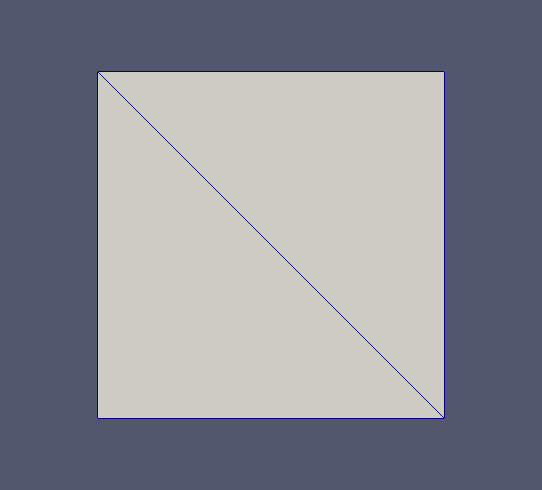
\includegraphics[width=0.8\textwidth]{distincttriangulation2.png}}}
\end{center}
\end{minipage}
\caption{sample of an edge flip}
\end{figure}
\end{center}

\indent Among all the triangulations of a certain point set, there are many circumstances in which certain triangulations are valued more highly than others. The Delaunay triangulation is an extremely important one. It has several equivalent definition from different points of sight. An accessible one is as follow:
\begin{myDef}\
For all triangles in a triangulation, if the circumcircle of that triangle has no points other than the three vertices inside, the triangulation is a Delaunay triangulation.
\end{myDef}
\indent This definition implies that the Delaunay triangulation provides the more regular triangles than other triangulations, which exactly the mesh necessitates for its quality.  Therefore, Delaunay based mesh generation methods are various, such as divide and conquer algorithm, incremental algorithm, get the dual graph of voronoi, and etc. In our strategy, the incremental algorithm based on lawson flip\cite{lawson}(the algorithm to transform a random triangulation into Delaunay via a selected sequence of edge flip) is used due to the flexibility as well as the robustness provided, even though the computational complexity is not the best.\\
\begin{algorithm}
\KwIn{\\A point set $S$\;}
\KwOut{\\A Delaunay triangulation $T$\;}
Randomly select 3 points to generate the first triangle.Remove the 3 points from $S$\;
\While{$S$ is not empty}{
Take one point,denoting $p$, and locate the point on current triangulation\;
\eIf{$p$ is in the convex hull of current triangulation}
{Call a 1-3 flip or 2-4 flip to insert the new point into the triangulation\;}
{Generate a new triangle with the proper edge on the convex hull and the new point\;}
Call the lawson flip to transform the new triangulation to Delaunay\;}
\caption{Delaunay triangulation generation algorithm}
\end{algorithm}
\indent Here the 1-3 flip and 2-4 flip refer to the point inserting strategy. If the point is in an triangle, then play a 1-3 flip transforming the triangle into 3 triangles. If the point locates on an edge of 2 triangles, then call a 2-4 flip transforming the 2 triangles into 4 triangles. Show in \ref{insert}.


\begin{center}
\begin{figure}[htbp]{\label{insert}}
\centering
\begin{minipage}[t]{0.4\linewidth}
\begin{center}
\subfigure{\label{flip1-3}}
\addtocounter{subfigure}{-2}
\subfigure[before 1-3 flip]{\subfigure{
\includegraphics[width=0.8\textwidth]{1-3.png}}}
\end{center}
\end{minipage}
\begin{minipage}[t]{0.4\linewidth}
\begin{center}
\subfigure{\label{flip1-3after}}
\addtocounter{subfigure}{-2}
\subfigure[after 1-3 flip]{\subfigure{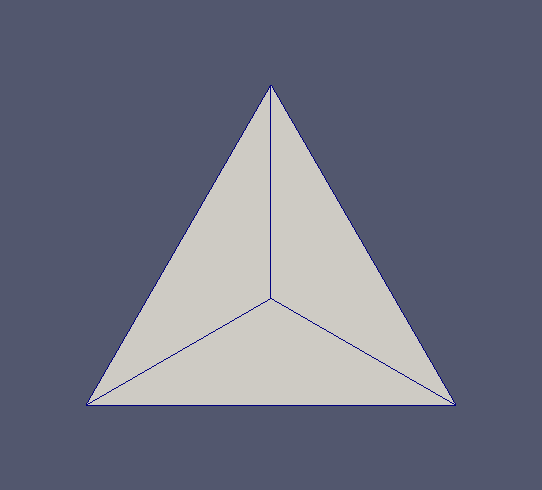
\includegraphics[width=0.8\textwidth]{1-3after.png}}}
\end{center}
\end{minipage}

\begin{minipage}[t]{0.4\linewidth}
\begin{center}
\subfigure{\label{flip2-4}}
\addtocounter{subfigure}{-2}
\subfigure[before 2-4 flip]{\subfigure{
\includegraphics[width=0.8\textwidth]{2-4.png}}}
\end{center}
\end{minipage}
\begin{minipage}[t]{0.4\linewidth}
\begin{center}
\subfigure{\label{flip2-4after}}
\addtocounter{subfigure}{-2}
\subfigure[after 2-4 flip]{\subfigure{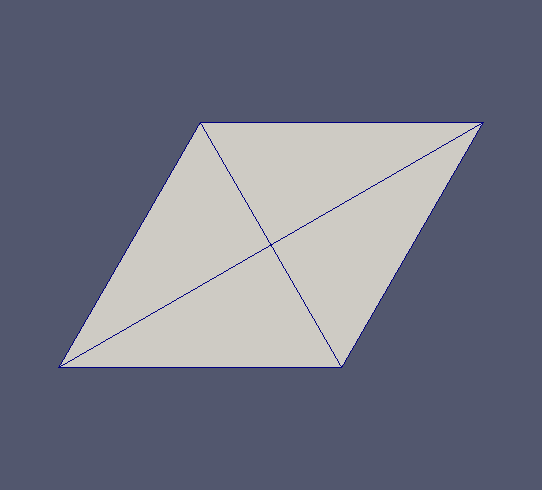
\includegraphics[width=0.8\textwidth]{2-4after.png}}}
\end{center}
\end{minipage}
\caption{Insert strategy}
\end{figure}
\end{center} 

\subsection{Constrained Delaunay triangulation and Delaunay refinement}
Delaunay triangulation provides an effective method generating quality mesh. Further more, the Delaunay triangulation of a certain point set is unique as long as the points are in general position,which means that no group of four points of are cocircular and no two points are in coincidence. However, in specific case, there may be some of the edges are necessary to form the boundary of the body while they are not in the Delaunay triangulation.Therefore, we have to constrain these edge to the final triangulation, which is called constrained Delaunay triangulation.\\
\indent Since the constrained Delaunay triangulation is global Delaunay with locally non-Delaunay, it is an effective way to generate a constrained Delaunay triangulation from the Delaunay triangulation via a series of flip to recover the constrained edge\cite{constrained1}.\\
\indent As for Delaunay refinement,it is a method to enhance the mesh quality via adding points outer from the original point set. Since the original point set may be non-uniform on the plane, even Delaunay triangulation may provide mesh with quite poor quality.For the time being, this method can be called to improve the quality via inserting extra points spliting big cell and causing flips to avoid small angle.Specificly, this procedure checks every triangles and insert points at the circlecenter of the too big ones,either, insert points at the constrained edges of the ones with too small angle\cite{refinement1}.By iterating the above procedure, the original Delaunay triangulation is refined and more uniformed.
\subsection{High dimensional embedding}
In \cite{hd embed}, Dassi, Si and Perotto provide a novel method for generating anisotropic mesh via high dimensional embedding.The main idea of this method is lift all the points into a high dimensional space,call embedding space, via an embedding function defined before. Then generate a quasi-Delaunay triangulation in this embedding space via a sequence of splitting , contracting and flipping of edges based on the embedding distance.Finally, project the quasi-Delaunay triangulation into the original plane.It is emphasized that the anisotropic property is inheriting from the embedding function.In other word, it is able to change the embedding function to view this method as an adaptive refinement algorithm.
\section{Dynamic mesh generation}
Our dynamic mesh generation strategy is based on the constrained Delaunay triangulation introduced in the last section.A series of consecutive constrained edge to represent the boundary of the body.The main quest is to move these edge to simulate the motion or deformation of the body.
\subsection{Overview of the algorithm}
Frankly speaking, the main idea of our grid-moving strategy is 'digging a hole' around the moving bodies to enable the motion of boundary without any intersection with other edges or points.After the movement of the boundary, lawson flip and delaunay refinement are called locally to refine the Delaunay property as well as the grid quality.\\
\begin{algorithm}
\KwIn{\\A point set $S$\\A series of vectors describing the motion of boundary points of each step $\{v_s^t\}$\\Max step $Maxstep$}
\KwOut{\\A series of meshes $\{M^t\}$}
Generate the triangulation of the first step\;
$step=0$\;
Output the triangulation as $M^{step}$\;
\While{$step<Maxstep$}{
Recover the segments from the refined triangulation by removing the free segment points\;
Remove the collision points and edges\;
Move the boundary edges via moving the constrained segment points $S_i^{step+1}=S_i^{step}+v_{S_i}^{step}$\;
Call locally lawson flip and locally Delaunay refinement\;
Output the triangulation as $M^{step}$\;
}
\caption{Dynamic mesh generation algorithm}
\label{DMGalgo}
\end{algorithm}
\indent This algorithm follows the commonsense of clear the barrier of moving objects. So that the objects can be moved directly without any collision. Since the algorithm employs removing and inserting of points, it is obvious an topology-changed dynamic mesh generation algorithm, which enables deformation,relative motion,and large displacement.Never the less, this generation strategy greatly decreases the time cost because no iteration is called in each step.
\subsection{Algorithm detail discussion}
In this subsection, the details of the above algorithm is discussed.\\
\indent Since the discription of boundary motion is restricted on the motion vectors at the constrained segment points, the free segment points must be removed to ensure the uniform of boundary edges and reduce the amount of triangles, which induces to the decrease of calculation.\\
\indent To remove the collision points, the collision points must be found out from the list of points first. According to the motion of each boundary edge, the points in the region it sweeping over are all collide to the edge. Therefore, it is able to remove the combine of collision points of all boundary edges. However, this strategy is computational inefficient since the search of collision points need to loop the full points list for each boundary edge.Thus, it is able to loose the criterion of collision points removing more points while decrease the search computation. In our case, a rectangle box,parelleling to coordinate, is employed covering the moving object and the place where it should move to. Moreover, to avoid too bad triangle after moving,the box is expand a little on each direction.Then it is able to loop only once within the points list to find out all the collision points according to this criterion. However,merely removing the collision points is not abundant beacuse collision edges may remain,shown in fig \ref{collision edge}.So to deal with the collision edges, it is available to flip all the collision edge from closer to further, to clear a way for moving the constrained segment points directly.\\
\indent After all the constrained segment points moved, the lawson flip and Delaunay refinement algorithm is called locally,to reduce the computational cost.Detailly, only the triangles adjacent to the constrained segment points are pushed into the flip queue as well as the refinement array.
\subsection{Dynamic high dimensional embedding}
To employ the high dimensional embedding algorithm into the dynamic mesh generation strategy, it is a trivial idea to modify the embedding function step by step, adjusting to the moving objects. Following this idea, the dynamic mesh generation strategy can be modified as locally lawson flip and Delaunay refinement replaced with high dimensional embedding function with dynamic embedding funciton.\\ 
\begin{algorithm}
\KwIn{\\A point set $S$\\A series of vectors describing the motion of boundary points of each step $\{v_s^t\}$\\Max step $Maxstep$\\Dynamic embedding funcition $F(x,y,t),\quad t=1,2,\cdots,Maxstep$}
\KwOut{\\A series of meshes $\{M^t\}$}
Generate the triangulation of the first step\;
$step=0$\;
Output the triangulation as $M^{step}$\;
\While{$step<Maxstep$}{
Recover the segments from the refined triangulation by removing the free segment points\;
Remove the collision points and edges\;
Move the boundary edges via moving the constrained segment points $S_i^{step+1}=S_i^{step}+v_{S_i}^{step}$\;
Dynamic high dimensional embedding\;
Output the triangulation as $M^{step}$\;
}
\caption{Dynamic mesh generation algorithm}
\label{DMGwithHDE}
\end{algorithm}
\indent This algorithem enable the generation of adaptive refined mesh along with dynamic generation, for instance, anisotropic grids around deformation boundary to simulate the boundary layer.
\section{Results}
\subsection{Deformation cases}
Subsection text here.
\subsection{Relative motion cases}


\subsubsection{}
Subsubsection text here.


% An example of a floating figure using the graphicx package.
% Note that \label must occur AFTER (or within) \caption.
% For figures, \caption should occur after the \includegraphics.
% Note that IEEEtran v1.7 and later has special internal code that
% is designed to preserve the operation of \label within \caption
% even when the captionsoff option is in effect. However, because
% of issues like this, it may be the safest practice to put all your
% \label just after \caption rather than within \caption{}.
%
% Reminder: the "draftcls" or "draftclsnofoot", not "draft", class
% option should be used if it is desired that the figures are to be
% displayed while in draft mode.
%
%\begin{figure}[!t]
%\centering
%\includegraphics[width=2.5in]{myfigure}
% where an .eps filename suffix will be assumed under latex,
% and a .pdf suffix will be assumed for pdflatex; or what has been declared
% via \DeclareGraphicsExtensions.
%\caption{Simulation results for the network.}
%\label{fig_sim}
%\end{figure}

% Note that the IEEE typically puts floats only at the top, even when this
% results in a large percentage of a column being occupied by floats.


% An example of a double column floating figure using two subfigures.
% (The subfig.sty package must be loaded for this to work.)
% The subfigure \label commands are set within each subfloat command,
% and the \label for the overall figure must come after \caption.
% \hfil is used as a separator to get equal spacing.
% Watch out that the combined width of all the subfigures on a
% line do not exceed the text width or a line break will occur.
%
%\begin{figure*}[!t]
%\centering
%\subfloat[Case I]{\includegraphics[width=2.5in]{box}%
%\label{fig_first_case}}
%\hfil
%\subfloat[Case II]{\includegraphics[width=2.5in]{box}%
%\label{fig_second_case}}
%\caption{Simulation results for the network.}
%\label{fig_sim}
%\end{figure*}
%
% Note that often IEEE papers with subfigures do not employ subfigure
% captions (using the optional argument to \subfloat[]), but instead will
% reference/describe all of them (a), (b), etc., within the main caption.
% Be aware that for subfig.sty to generate the (a), (b), etc., subfigure
% labels, the optional argument to \subfloat must be present. If a
% subcaption is not desired, just leave its contents blank,
% e.g., \subfloat[].


% An example of a floating table. Note that, for IEEE style tables, the
% \caption command should come BEFORE the table and, given that table
% captions serve much like titles, are usually capitalized except for words
% such as a, an, and, as, at, but, by, for, in, nor, of, on, or, the, to
% and up, which are usually not capitalized unless they are the first or
% last word of the caption. Table text will default to \footnotesize as
% the IEEE normally uses this smaller font for tables.
% The \label must come after \caption as always.
%
%\begin{table}[!t]
%% increase table row spacing, adjust to taste
%\renewcommand{\arraystretch}{1.3}
% if using array.sty, it might be a good idea to tweak the value of
% \extrarowheight as needed to properly center the text within the cells
%\caption{An Example of a Table}
%\label{table_example}
%\centering
%% Some packages, such as MDW tools, offer better commands for making tables
%% than the plain LaTeX2e tabular which is used here.
%\begin{tabular}{|c||c|}
%\hline
%One & Two\\
%\hline
%Three & Four\\
%\hline
%\end{tabular}
%\end{table}


% Note that the IEEE does not put floats in the very first column
% - or typically anywhere on the first page for that matter. Also,
% in-text middle ("here") positioning is typically not used, but it
% is allowed and encouraged for Computer Society conferences (but
% not Computer Society journals). Most IEEE journals/conferences use
% top floats exclusively.
% Note that, LaTeX2e, unlike IEEE journals/conferences, places
% footnotes above bottom floats. This can be corrected via the
% \fnbelowfloat command of the stfloats package.




\section{Conclusion}
The conclusion goes here.




% conference papers do not normally have an appendix


% use section* for acknowledgment
\section*{Acknowledgment}


The authors would like to thank...





% trigger a \newpage just before the given reference
% number - used to balance the columns on the last page
% adjust value as needed - may need to be readjusted if
% the document is modified later
%\IEEEtriggeratref{8}
% The "triggered" command can be changed if desired:
%\IEEEtriggercmd{\enlargethispage{-5in}}

% references section

% can use a bibliography generated by BibTeX as a .bbl file
% BibTeX documentation can be easily obtained at:
% http://mirror.ctan.org/biblio/bibtex/contrib/doc/
% The IEEEtran BibTeX style support page is at:
% http://www.michaelshell.org/tex/ieeetran/bibtex/
%\bibliographystyle{IEEEtran}
% argument is your BibTeX string definitions and bibliography database(s)
%\bibliography{IEEEabrv,../bib/paper}
%
% <OR> manually copy in the resultant .bbl file
% set second argument of \begin to the number of references
% (used to reserve space for the reference number labels box)
\begin{thebibliography}{1}
\bibitem{60}
Zhe Jiang. Research of the Generation of Dynamic Unstructured Meshes[D]. Nanjing University of Science \& Technology, 2006.
\bibitem{hd embed}
Dassi F, Si H, Perotto S, et al. Anisotropic Finite Element Mesh Adaptation via Higher Dimensional Embedding[J]. Procedia Engineering, 2015, 124:265-277.
\bibitem{Discrete}
Devadoss S L, O'Rourke J. Discrete and computational geometry[M]. Springer, 2001.
\bibitem{lawson}
Charles Lawson. Transforming triangulations. Discrete Mathematics, Volume 3, pages 365�C372, 1972.
\bibitem{constrained1}
Chew L P. Constrained Delaunay triangulations[J]. Algorithmica, 1989, 4(1-4):97-108.
\bibitem{constrained2}
Shewchuk, Jonathan R. (2008). "General-Dimensional Constrained Delaunay and Constrained Regular Triangulations, I: Combinatorial Properties". 39 (1-3): 580�C637.
\bibitem{refinement1}
Ruppert, Jim (1995). "A Delaunay refinement algorithm for quality 2-dimensional mesh generation". Journal of Algorithms. 18 (3): 548�C585. doi:10.1006/jagm.1995.1021
\end{thebibliography}




% that's all folks
\end{document}


